\section{EXP10 stochastic robustness}
\label{sec:or1-exp10}

\subsection{Design}

93-instance common sparse subset; 20 IPSNS seeds (0--19); 20 DRMacIver/FAS repetitions per instance. Production records: 1860+1860 validated (0 failures). Smoke artifacts excluded.

\subsection{Primary median comparison}

\begin{center}
\begin{tabular}{lr}
\toprule
Metric & Value \\
\midrule
IPSNS wins / ties / DR wins & 38 / 55 / 0 \\
Mean relative excess (DR over IPSNS) & 21.60\% \\
Wilcoxon $p$ (two-sided) & $<0.001$ \\
Sign test $p$ (two-sided) & $<0.001$ \\
Cohen's $d_z$ & $-0.31$ \\
\bottomrule
\end{tabular}
\end{center}

\subsection{Variability}

IPSNS: zero objective variation on 93/93 instances; seed 0 matched best on all 93. DRMacIver: 40/93 instances with multiple distinct objectives; 1860 unique PIDs.

\subsection{\texttt{r20\_60} reversal}

EXP4 single run: DRMacIver 1685 vs IPSNS 1688 (DR win). EXP10 medians: IPSNS 1688 vs DRMacIver 1698 (IPSNS win).

\subsection{Warnings}

\begin{itemize}
  \item Zero IPSNS cross-seed variance documents empirical stability under the frozen configuration; it does \textbf{not} prove mathematical determinism.
  \item The repeated-run comparison is \textbf{not} equal-time; DRMacIver intermediate solutions are unavailable.
\end{itemize}

\subsection{Figures and tables}

\begin{figure}[h]
\centering
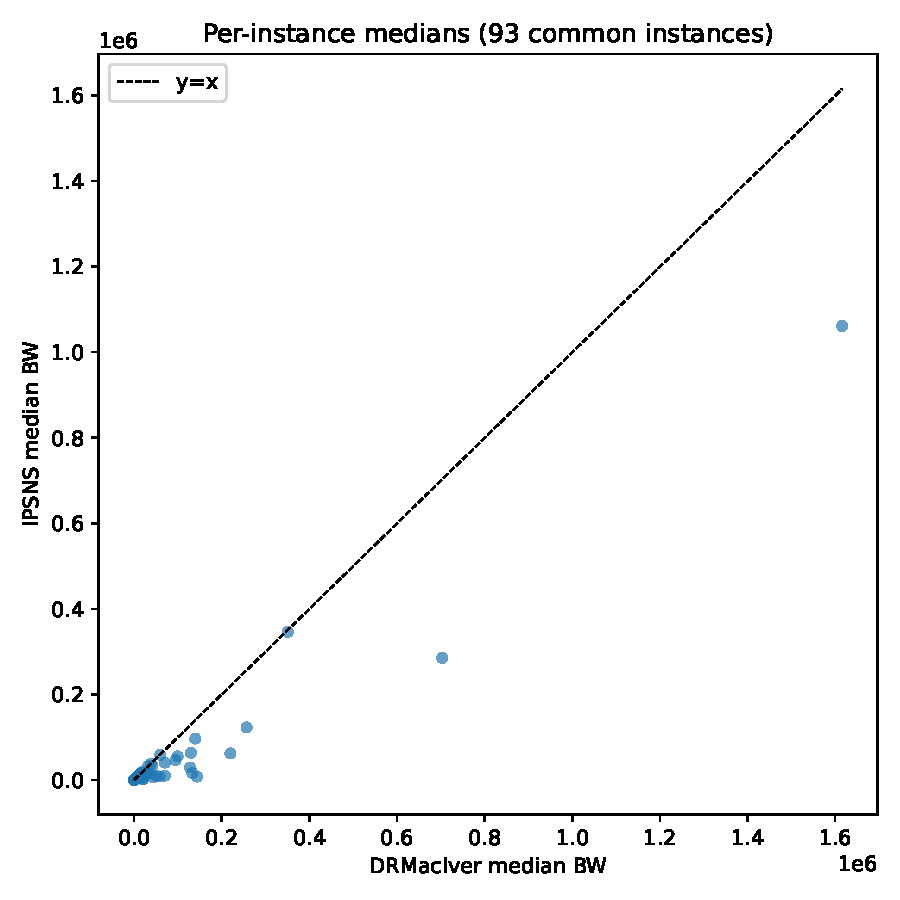
\includegraphics[width=0.55\textwidth]{figures/exp10_median_scatter.pdf}
\caption{EXP10 per-instance medians (93 instances).}
\end{figure}

Complete tables: \texttt{results/exp10/summary/paired\_median\_comparison.csv}, \texttt{best\_of\_k.csv}, \texttt{probability\_of\_win.csv}. Figures: \texttt{results/exp10/figures/}.
